\documentclass{llncs}

\usepackage[utf8]{inputenc}
\usepackage[T1]{fontenc}
\usepackage[noadjust,nosort]{cite}
\usepackage[fleqn]{amsmath}
\usepackage{amsfonts}
\usepackage{amssymb}
%\usepackage{MnSymbol}
%\usepackage{thmtools}
%\usepackage{thm-restate}
\usepackage{booktabs}
\usepackage{figlatex}
\usepackage{xcolor}
\usepackage{setspace}
\usepackage{xspace}
\usepackage[super]{nth}
\usepackage{multicol}
\usepackage{microtype}
\usepackage{wrapfig}
\usepackage{graphicx}
\usepackage{subfig}
\usepackage{comment}
\usepackage[center,width=152mm,height=235mm]{crop}
%\usepackage[pagewise,switch]{lineno} % switch, modulo, pagewise
\usepackage{hyperref}
%\usepackage[linesnumbered,lined,noend,ruled]{algorithm2e}
\usepackage[lined,noend,ruled]{algorithm2e}
%\usepackage{algorithmic}
\usepackage[noend]{algpseudocode}
\usepackage[capitalise,english,nameinlink]{cleveref} % load after algorithm2e and hyperref

\hypersetup{
	bookmarksdepth=2,
	bookmarksnumbered=true,
	bookmarksopen=true,
	bookmarksopenlevel=2,
	colorlinks=true,
	linktocpage=true,
	breaklinks=true,
	pageanchor=true,
	allcolors=[rgb]{0.6,0.0,0.0},
	pdftitle={DPU's data structures and algorithms},
	pdfauthor={Huyen N.T.T, César Rodríguez}
}

%\newcommand\comp {\mathfrak{c}}
%\newcommand\cycles[1]  {\mathsf{Cycles}{(#1)}}
%\newcommand\extn {\mathcal{X}}
%\newcommand\lchist[2]  {{ {#1}\langle#2\rangle }}
%\newcommand\lonepref   {\ppref^1_{N}}
%\newcommand\lpg     {\leadsto_\config}
%\newcommand\lstruc  {\mathcal{L}}
%\newcommand\ltwopref   {\ppref^2_{N}}
%\newcommand\maxspoilers[1]{t^{\spoils}_{#1}}
%\newcommand\move[1] {\stackrel{#1}{\longrightarrow }}
%\newcommand\myleq   \le
%\newcommand\nat     {\mathrm{I\!N}}
%\newcommand\node[1] {\mathit{#1}}
\newcommand\pac      {\mathrel{\nearrow\!\!\!\!\!\nearrow}}
\newcommand\rd       \propto
%\newcommand\spoils  {\dagger}

% relations
%\newcommand\reveals  {\mathrel{\triangleright}}
%\newcommand\ac       {\mathrel{\nearrow}}
\newcommand\aco      {\mathrel{/\!\!/}}
\newcommand\cfl      {\mathrel{\#}}
\newcommand\icfl[1][]{\mathrel{\#^i_{#1}}}
\newcommand\co       {\mathrel{\parallel}}
\newcommand\indep    {\mathrel{\meddiamond}}
\newcommand\depen    {\mathrel{\diamondtimes}}
\newcommand\eqdef    {\mathrel{:=}}
\newcommand\evolves  {\mathrel{\sqsubseteq}}
\newcommand\evstrict {\mathrel{\sqsubset}}
\newcommand\ispref   {\mathrel{\trianglelefteq}}
\newcommand\icause   {\mathrel{<_i}}
\newcommand\ifft     {\mathrel{\text{ iff }}}
\newcommand\nco      {\mathrel{\not\!\!\;\,\co}}
\newcommand\fire[1]  {\mathrel{\raisebox{-1.1pt}{$\xrightarrow{#1}$}}}

\newcommand\extreveals  {\mathbin{-\hspace{-2.5mm}-\hspace{-2.0mm}\reveals}}

% operators
\newcommand\iscutoff[1] {\mathop{\mathsf{cutoff}} (#1)}
\newcommand\union[1]    {\mathop{\mathit{union}} (#1)}
\newcommand\merge[1]    {\mathop{\mathfrak{Merge}} (#1)}
\newcommand\od[1]       {\mathop{\mathrm{od}} (#1)}
\newcommand\amo[1]      {\mathop{\textsf{AMO}} (#1)}
\newcommand\acyclic[1]  {\mathop{\textsf{ACY}} (#1)}
\newcommand\bigo[1]     {\mathop{\mathcal{O}} (#1)}
\newcommand\progloop[1] {\mathop{\mathit{ploop}} (#1)}
\newcommand\allhist[1]  {\mathop{\mathit{Hist}} (#1)}
\newcommand\compt[1]    {\mathop{\mathit{compat}} (#1)}
\newcommand\conc[1]     {\mathop{\mathit{conc}} (#1)}
\newcommand\conf[1]     {\mathop{\mathit{conf}} (#1)}
\newcommand\cut[1]      {\mathop{\mathit{cut}} (#1)}
\newcommand\explain[1]  {\mathop{\mathit{expl}} (#1)}
\newcommand\lpo[1]      {\mathop{\mathit{lpo}} (#1)}
\newcommand\marking[1]  {\mathop{\mathit{mark}} (#1)}
\newcommand\obser[1]    {\mathop{\mathit{obs}} (#1)}
\newcommand\peel[2]     {\mathop{\mathit{peel}}_{#2} (#1)}
\newcommand\peelast[1]  {\mathop{\mathit{peelmax}} (#1)}
\newcommand\reach[1]    {\mathop{\mathit{reach}} (#1)}
\newcommand\runs[1]     {\mathop{\mathit{runs}} (#1)}
\newcommand\sfp[1]      {\mathop{\mathit{pred}} (#1)}
\newcommand\spoilers[1] {\mathop{\mathit{spoilers}} (#1)}
\newcommand\state[1]    {\mathop{\mathit{state}} (#1)}
\newcommand\succexpl[1] {\mathop{\mathit{succexpl}} (#1)}
\newcommand\trim[2]     {\mathop{\mathit{trim}_{#2}} (#1)}
\newcommand\trimast[1]  {\mathop{\mathit{trimmax}} (#1)}
\newcommand\depth[1]    {\mathop{\mathit{depth}} (#1)}
\newcommand\pe[1]       {\mathop{\mathit{pe}} (#1)}
\newcommand\inter[1]    {\mathop{\mathit{inter}} (#1)}
\newcommand\proc[1]     {\mathop{\mathit{proc}} (#1)}
\newcommand\enabl[1]    {\mathop{\mathit{enabl}} (#1)}
\newcommand\en[1]       {\mathop{\mathit{en}} (#1)}
\newcommand\ex[1]       {\mathop{\mathit{ex}} (#1)}
\newcommand\cex[1]      {\mathop{\mathit{cex}} (#1)}
\newcommand\fcfl[1]     {\mathop{\mathit{\#}} (#1)}
\newcommand\ficfl[2][]  {\mathop{\mathit{\#^i_{#1} }} (#2)}
\newcommand\forml[1]    {\mathcal{L} (#1)}

\newcommand\mult[1]     {\mathbf{#1}}
\newcommand\sem[1]      {\mathrm{[\![{#1}]\!]}}
\newcommand\hist[2]     {{ {#1}[\![#2]\!] }}
\newcommand\cont[1]     {\underline{#1}}
\newcommand\post[1]     {#1^\bullet}
\newcommand\pre[1]      {{}^\bullet#1}
\newcommand\support[1]  {\bar{#1}}
\newcommand\causes[1]   {\left \lceil #1 \right \rceil}
\newcommand\future[1]   {\left \lfloor #1 \right \rfloor}

\newcommand\FIXME[1]    {\textcolor{red}{\texttt{FIXME: #1}} }
\newcommand\anc[1]      {{#1}^\uparrow}
\newcommand\eenr        {\mathcal{E}}
\newcommand\enr[1]      {\mathcal{E}_{#1}}
%\newcommand\pes         {\mathcal{E}}
\newcommand\les         {\mathcal{E}}
\newcommand\unf[1]      {\mathcal{U}_{#1}}
\newcommand\unr[1]      {\mathcal{M}_{#1}}
\newcommand\var[1]      {\mathsf{#1}}
\newcommand\mer[1]      {\mathcal{Q}_{#1}}
\newcommand\hst[1]      {\mathcal{H}_{#1}}
\newcommand\trunc[1]    {\mathcal{T}_{#1}}
\newcommand\htrunc[1]   {\widehat{\mathcal{T}}_{#1}}
\newcommand\pref[1]     {\mathcal{P}_{#1}}
\newcommand\precpref[1] {\mathcal{P}^\prec_{#1}}
\newcommand\trace[1]    {\mathcal{T}_{#1}}
\newcommand\dgraph[1]   {\mathcal{D}_{#1}}
\newcommand\intsem[1]   {\mathcal{S}_{#1}}
\newcommand\cutoffs     {\mathcal{K}}

% abbreviations
\newcommand\precutoff{\text{$\prec$-cutoff}}
\newcommand\phiasym  {\phi_\ppref^\text{asym}}
\newcommand\phicausal{\phi_\ppref^\text{causal}}
\newcommand\phiconf  {\phi_\ppref^\text{conf}}
\newcommand\phidead  {\phi_\ppref^\text{dead}}
\newcommand\phidis   {\phi_\ppref^\text{dis}}
\newcommand\phimark  {\phi_\ppref^{\text{mark},M}}
\newcommand\phicov   {\phi_\ppref^{\text{cov},M}}
\newcommand\phip     {\phi_\ppref}
\newcommand\phisym   {\phi_\ppref^\text{sym}}

\newcommand\mphimark {\gamma_\qpref^{\text{mark},M}}
\newcommand\mphicon  {\gamma_\qpref^{\text{con},M}}
\newcommand\mphiaux  {\gamma_\qpref^\text{aux}}
\newcommand\mphiflow {\gamma_\qpref^\text{flow}}
\newcommand\mphiasym {\gamma_\qpref^\text{asym}}
\newcommand\mphicov  {\gamma_\qpref^{\text{cov},M}}
\newcommand\mphigap  {\gamma_\qpref^\text{no-gap}}
\newcommand\mphipath {\gamma_\qpref^\text{path}}

\newcommand\mphiconf {\gamma_\qpref^\text{conf}}
\newcommand\mphidis  {\gamma_\qpref^\text{dis}}
\newcommand\mphip    {\gamma_\qpref}


\newcommand\mcitomp  {\textsc{Mci2mp}\@\xspace}
\newcommand\minisat  {\textsc{Minisat}\@\xspace}
\newcommand\mole     {\textsc{Mole}\@\xspace}
\newcommand\prcompress{\textsc{PRCompress}\@\xspace}
\newcommand\clp      {\textsc{Clp}\@\xspace}
\newcommand\cmerge   {\textsc{Cmerge}\@\xspace}
\newcommand\cunf     {\textsc{Cunf}\@\xspace}
\newcommand\poet     {\textsc{Poet}\@\xspace}
\newcommand\nidhugg  {\textsc{Nidhugg}\@\xspace}
\newcommand\cosyverif{\textsc{Cosyverif}\@\xspace}
\newcommand\coloane  {\textsc{Coloane}\@\xspace}
\newcommand\tapaal   {\textsc{Tapaal}\@\xspace}
\newcommand\cunft    {Cunf~Toolset}
\newcommand\cna      {\textsc{Cna}\@\xspace}
\newcommand\punf     {\textsc{Punf}\@\xspace}
\newcommand\salpha   {\ppref_\alpha}
\newcommand\spcutoff {\text{sp-cutoff}}
\newcommand\id       {\textit{id}}
\newcommand\ep       {EP}
\newcommand\dr       {Dr.\@\xspace}
\newcommand\mr       {Mr.\@\xspace}
\newcommand\prof     {Prof.\@\xspace}

\newcommand\uunf     {\mathcal{U}}
\newcommand\ppref    {\mathcal{P}}
\newcommand\qpref    {\mathcal{Q}}
\newcommand\con      {\mathcal{C}}
\newcommand\N        {\mathbb{N}}
\newcommand\Q        {\mathbb{Q}}
\newcommand\R        {\mathbb{R}}
\newcommand\obs      {\mathbb{O}}
\newcommand\hhat     {\widehat h}
\newcommand\ehat     {\widehat e}
\newcommand\chat     {\widehat c}
\newcommand\conhat   {\widehat \con}
\newcommand\Hhat     {\widehat H}
\newcommand\Ehat     {\widehat E}
\newcommand\Bhat     {\widehat B}
\newcommand\cgen     {\var{c_{\text{gen}} }}
\newcommand\cpgen    {\var{c'_{\text{gen}} }}
\newcommand\ccon     {\var{c_{\text{con}} }}
\newcommand\ccut     {\var{c_{\text{cut}} }}

\newcommand\pp       {pp.\@\xspace}
\newcommand\viz      {viz.\@\xspace}
\newcommand\vs       {vs.\@\xspace}
\newcommand\wlogg    {w.l.o.g.\xspace}
\newcommand\aka      {a.k.a.\xspace}
\newcommand\wrt      {w.r.t.\@\xspace}
\newcommand\cf       {cf.\@\xspace}
\newcommand\Wlog     {W.l.o.g.\xspace}
\newcommand\al       {al.\@\xspace}
\newcommand\eg       {e.g.\@\xspace}
\newcommand\etc      {etc.\@\xspace}
\newcommand\ie       {i.e.\@\xspace}
\newcommand\naive    {na{\"\i}ve\xspace}
%\newcommand\st      {s.t.\@\xspace}
\newcommand\resp     {resp.\@\xspace}
\newcommand\nr       {nr.\@\xspace}
\newcommand\avg      {avg.\@\xspace}

% miscellaneous
\newcommand\cod[1]   {\texttt{#1}}
\newcommand\tup[1]   {\langle#1\rangle}
\newcommand\set[1]   {{\{ #1 \mathclose \}}}
\newcommand\eqtag[1] {\hfill{} \refstepcounter{equation} \label{#1} (\arabic{equation})}

%\newtheorem{cor} {Corollary}
%\newtheorem{defn}   {Definition}
%\newtheorem{lemma}  {Lemma}
%\newtheorem{proposition}{Proposition}
%\newtheorem{remark} {Remark}
%\newtheorem{theorem}   {Theorem}

%\renewcommand{\algorithmicensure}{\textbf{Output}:}
%\renewcommand{\algorithmicrequire}{\textbf{Input}:}
%\renewcommand{\labelitemi}{\textbf{--}}
%\renewcommand{\labelitemi}{{\footnotesize $\bullet$}}

% e  equation
% d  def
% f  figure
% l  lemma, line
% s  section
% r  remark
% p  proposition
% t  theorem
% c  corollary
% b  table
% a  algorithm
% x  appendix
% h  chapter
% n  footnote
% m  example

% for standard names
\crefname{equation}{}{}
\crefname{proposition}{Prop.}{Props.}
\Crefname{proposition}{Proposition}{Propsitions}
\crefname{section}{\S}{\S\S}
\Crefname{section}{Section}{Sections}
\crefname{page}{p.}{pp.}
\Crefname{page}{Page}{Pages}
\crefname{chapter}{Ch.}{Ch.}
\Crefname{chapter}{Chapter}{Chapters}
\crefname{remark}{Rmk.}{Rmks.}
\Crefname{remark}{Remark}{Remarks}
\crefname{appendix}{App.}{App.}
\Crefname{appendix}{Appendix}{Appendix}
\crefname{algorithm}{Alg.}{Alg.}
\Crefname{algorithm}{Algorithm}{Algorithms}
%\crefname{algocf}{algorithm}{algorithm}
%\Crefname{algocf}{Algorithm}{Algorithm}
\crefname{line}{line}{line}
\Crefname{line}{Line}{Line}

% for LIPICs
\crefname{theo}{Theorem}{Theorems}
\crefname{lem}{Lemma}{Lemmas}
\crefname{cor}{Corollary}{Corollaries}
\crefname{prop}{Prop.}{Props.}
\crefname{defn}{Def.}{Defs.}
\Crefname{defn}{Definition}{Definitions}
\crefname{exampl}{Example}{Examples}
\crefname{rmk}{Remark}{Remarks}

%\crefname{AlgoLine}{algorithm}{algorithm}





\title{DPU Implementation Specification}
\author{Huyen Nguyen}
\institute{Université Paris 13, Sorbonne Paris Cité, LIPN, CNRS, France}

\begin{document}
\maketitle
\noindent
%\chapter{Execution Model}
Constructing the unfolding for a sytem is actually an exploration of all possible configurations from an input model.
\begin{itemize}
	\item
	 Input: A model M is described in terms of:
	 \begin{itemize}
	 	\item
		 	\verb!S!: A set of states where each one implies the states of all processes and variables of the system. Every system always has an well-defined initial state.
	 	\item
			\verb!T!: A set of transitions, one of who implies the system movement from one state to another.
	 	\item 
		 	\verb!P!: A set of processes with locations, transitions between them.
		
	 \end{itemize} 
	\item Output: A full unfolding with events labelled with transitions and relations including causality, conflict and concurrency.
\end{itemize}

\section{Execution Model}
\label{s:model}
\subsection{Data Structure}
\verb!Machine!: A class models a system in terms of:
	\begin{itemize}
	\item
		\verb!procs!: a vector (std::vector) of threads which are instances of \verb!Process! class
	\item
		\verb!trans!: a vector of transitions in all processes, instances of \verb!Transition! class 
	\item
		\verb!memsize!:	an \verb!int! number which is the size of memory dedicated to store the states of processes and
		 value of variables
	\item
		\verb!init_state!: a private initial state of system, an instance of \verb!State! class. This can be set up 
		by \verb!change_init_state! method
	\end{itemize}	


\subsection{Relevant classes}
Classes neccessary to model a system are State, Trans, Process:
\begin{enumerate}
\item
	\verb!State!: implies the state associated with a Machine $m$. The unique attribute \verb!tab! is an array of \verb!uint32_t! storing the process locations and variable values (including global and local variables) at the state. Its size is \verb!m.memsize!
\item
	\verb!Process!: A process is specified as:
	\begin{itemize}
	\item
		A vector of Trans instances
	\item
		A vector (std::vector) of vectors of \verb!Trans! indicates the control flow graph of the process
	\end{itemize}	 
\item
	\verb!Trans!: includes a numerous properties:
	\begin{itemize}
	\item
		\verb!proc!: process a transition belongs to.
	\item
		\verb!src!: source of transition which implies the process location enabling transition
	\item
		\verb!dest!: the target (a new location) process should reach when the transitions is fired.
	\item
		\verb!var!: an $int$ number implying address in memory area of the only global variable which is touched by transition (\verb!tab! of \verb!State!)
	\item
		\verb!offset!: the offset address from the variable which is helpful just in case \verb!var! is an array.
	\item
		\verb!localvars!: a vector of local variables which are read or written by transition
	\item
		\verb!code!: an instance of Codeblock class, a source code associated with a transition which can be any statement in C
		 programming language.
	\item
		\verb!type!: type of transition which can be read, write, synchronous or local. 
		Transition types :
		\begin{itemize}
		\item
			\verb!RD! Represents a transition that performs a certain amount of local (independent) work plus a single read
			 operation on some global variable.
		\item
			\verb!WR! Represents a transition that performs a certain amount of local (independent) work plus a single write
			 operation on some global variable.
		\item
			\verb!LOC! Represents a transition that only performs local (independent) operations.
		\item
			\verb!SYN! Represents a synchronization operation, intended to model a lock or unlock operation on a mutex.
		\end{itemize}
		
	\end{itemize}
	
\noindent	
Importan methods:
	\begin{itemize}
	\item
		\verb!enable(State s)!: a function returns $true$ if the transition is enabled at the state $s$ 
	\item
		\verb!fire(State s)!: fire the transition from $s$ providing that $s$ is asserted to enable the calling transition.
	\end{itemize}
\end{enumerate}

\section{Unfolding}
\label{s:unf}
\subsection{Data Structure}
	A vector of \verb!Event!s, a pointer to the bottom event, and a reference to the \verb!Machine!.

\subsection{Relevant classes}
To represent and construct an unfolding, we need some classes including Config, Event, Node, Multinode:
\begin{enumerate}
\item
	\verb!Config!: a configuration represents a set of conflict-free and causal closed events in a unfolding.
	\begin{itemize}
	\item
		\verb!gstate!: the state which is reached by firing sequentially events in the configuration.
	\item
		\verb!latest_proc!: a vector of pointers refering to the latest event in processes, so its size is the number of
		 processes.
	\item
		\verb!latest_wr!: a vector of pointers refering to the latest event writing on a variable. Its size is equal to the
		 number of variables.
	\item
		\verb!latest_op!: a vector of vectors of pointers indicateing the latest event in each process which reads or writes on
		a variable. its size is the number of processes multiplied by the \verb!memsize! of input machine $m$.
	\item
		\verb!en!: a vector of pointers to those who are enabled at the state of the configuration.
	\item
		\verb!cex!: a vector of pointer to those who are enabled at some sub-configuration of C and conflict with some event in
		 C
	\end{itemize}
\item
	\verb!Event!: the most important class in the unfolding which contains almost all neccessary information. Events represent the occurrence of transitions.
They store pointers to all their immediate causal predecessors (ICPs), and some of
the immediate causal successors (ICSs).
The number of ICPs is determined by the type of the transition they
represent:

\begin{itemize}
\item \verb!LOC! events: 1 predecessor (process)
\item \verb!SYN! events: 2 predecessors (process, last \verb!SYN! on same variable)
\item \verb!RD!  events: 2 predecessor (process + last \verb!RD! or
	\verb!WR! operation on the same variable)
\item \verb!WR!  events: 1 predecessor (process) + one predecessor per
	process (last \verb!RD! or \verb!WR! operation on that process)
\end{itemize}

The immediate causal successors of one event are determined by those events
for which the event is an immediate causal predecessor. Some of the causal
successors are stored in the \verb!Event! class, but not all.

All kinds of events store:
\begin{itemize}
\item
  \verb!trans!: a pointer to the transition it represents.
\item
  \verb!localvars!: vector (\verb!std::vector!) of \verb!uint32_t! values
  containing the value of the variables whose addresses are strored in
  \verb!this->trans->localvars!.
\item
  \verb!pre_proc!: (ICP) a pointer to the last event in the same thread.
\item
  \verb!post_proc!: (ICSs) a vector (\verb!std::vector!) of pointers to
  the next events in the same thread.
\end{itemize}
%
For \verb!SYN! events :
\begin{itemize}
\item
  \verb!pre_mem!: (ICP) pointer to the last \verb!SYN! event on the same
  variable, possibly performed by the same thread or another thread.
  Recall that \verb!SYN! operations on the same variable induce a tree when
  regarded unfolding-wise, and a total order (a branch of that tree) when
  the attention is reduced to an arbitrary configuration.
  In this regard, \verb!pre_mem! is a pointer to the node's parent in that
  tree.
\item
  \verb!post_mem!: (ICSs) vector (\verb!std::vector!) of pointers to
  the immediate next \verb!SYN! operations on the same variable, in this or
  another thread. These are the children of the aforementionned
  unfolding-wise tree.
\item
  \verb!val!: the value written by this event to the variable \verb!trans->var!
\end{itemize}
%
For \verb!RD! events :
\begin{itemize}
\item
  \verb!pre_mem!: (ICP) pointer to the last \verb!RD! or \verb!WR! event of
  the same thread. Observe that we do not store anything in the
  \verb!post_mem! vector.
\end{itemize}
%
Finally, for \verb!WR! events :
\begin{itemize}
\item
  \verb!pre_mem!: (causal predecessor) pointer to the last event
  representing a \verb!WR! operation performed on the same variable.
  Recall that \verb!WR! operations on the same variable induce a tree when
  regarded unfolding-wise, and a total order (a branch of that tree) when
  the attention is reduced to an arbitrary configuration.
  In this regard, \verb!pre_mem! is a pointer to the node's parent in that
  tree.
\item
	
  \verb!post_wr!: (causal WR successsor) vector (\verb!std::vector!) of
  pointers to the next \verb!WR! operations on the same variable, in this
  or another thread. These are the children of the aforementionned
  unfolding-wise tree.(need re-considered its existence)
\item
  \verb!post_mem!: (causal RD, SYN, WR immediate successors) a vector of vectors (\verb!std::vector<std::vecotr>!) of operations on the same variable in differents threads. 
	
\item
  \verb!pre_readers!: (immediate and not immediate causal predecessors)
  vector (\verb!std::vector!) of pointers to events (one per thread).
  The event pointed is the last \verb!RD! or \verb!WR! operation on the
  same variable performed in that thread.
\end{itemize}

\item
	\verb!MultiNode!
\item
	\verb!Node!

\end{enumerate}

\section{Event and Conflict}
\subsection{Immediate conflict}
Two events $e$ and $e'$ are in \textit{immediate conflict} $e \icfl e' $ iff $e \cfl e'$ and both $[e] \cup \lceil e' \rceil$ and $ \lceil e \rceil \cup [e']$ are configuration. Saying non-mathematically, they share one of their immediate predecessors, so-called parents.
Therefore, two events are in conflict only if they satisfy two condition:
\begin{itemize}
\item
	\textit{They have at least one parent in common which means they both are successors of an event.}
\item
	\textit{The union of their local configuration must be also a configuration.}
\end{itemize}

For alternative algorithm, in \verb!Event!, direct conflict events is stored as a vector of events, \textit{dicfl} which is updated whenever an event is created in the unfolding or others' appearances influenced on its relations.
An event can be created in two cases:
\begin{enumerate}
\item
	When a transition is enabled at a configuration, a corresponding event labelled with it is
	created and added to the configuration's enable set. By that time, we need to update $dicfl$ for 
	the new one.
\item
	In the time of computing conflict extension, a new event conflicting with an event $e$, labelled
	with transition $t$, is created by combining \verb!e.pre_proc! and new \verb!pre_mem! and 
	\verb!pre_readers!(See \cref{subsec:cex} for more details)	
\end{enumerate}

We propose two different algorithms to decide the direct conflict for these two cases.

\subsubsection{Checking direct conflict between two enable events.}
Given $e$ and $e'$ both enabled at a configuration $C$, $e, e' \in en(C)$, we have a lemma.
	
	\begin{lemma}{Direct conflict between enable events}
		\begin{itemize}
			\item
			$e$ and $e'$ are both in en(C), $e \icfl e'$ iff they share at least one parent.		
		\end{itemize}
		\label{thm:lem1}
	\end{lemma}
	
	\begin{proof}
	Two ways.
		\begin{itemize}
		\item
			($\leftarrow$) $e$ and $e'$ have a common parent $\rightarrow$ $e \icfl e'$
			
			$e$ and $e'$ sharing one parent means that  $e \cfl e'$. Moreover, $e$ and $e'$ are both 
			in en(C), so we have:
			\begin{itemize}
			\item
				$\lceil e \rceil \cup e'$ is a configuration.
			\item
				$\lceil e' \rceil \cup e$ is a configuration.
			\end{itemize} 
			According to the definition of direct conflict, it is obvious that $e \icfl e'$.
			
		\item
			($\rightarrow$) $e \icfl e'$ $\rightarrow$ they have at least one parent in common.
			
			Assume that $e$ and $e'$ share no parent, because $\lceil e \rceil \cup e'$ and $\lceil
			e' \rceil \cup e$ are configurations, $e || e'$ which means $\lnot (e \cfl e')$
		\end{itemize}			
	\end{proof}			
	
	\noindent
	Thank to \autoref{thm:lem1}, to decide if $e$ and $e'$ are in conflict, we just need to check if
	they are both successors of an event, which means their appearances in \verb!post_mem! of one 
	parent.
	Notice that they are in a enable set of configuration, so they cannot have the same 
	\verb!pre_proc! (The system is deterministic). To determine immediate conflict between two
	events $e$ and $e'$, do as follows: 
	\begin{itemize}
	\item
		One of them is a LOC, there is definitely no conflict between them at all.
	\item
		If they have the same predecessor \verb!e.pre_proc = e'.pre_proc!, they are in the same
		process as well as have the same source which implies they conflict.
	\item
		If they are in different processes (have different \verb!pre_proc!), look at one's 
		\verb!parent! which will be \verb!e.pre_mem! 		if $e$ is a RD or SYN (We can do the
		same to $e'$ when $e$ is a WR and $e'$ is a RD or SYN). The case of two WRs will be
		seperately treated.
		\begin{itemize}
		\item
			\verb!parent! is RD or SYN: if we find $e'$ in \verb!parent.post_rws!, then they are in
			conflict.
		\item
			\verb!parent! is WR or bottom: if we find $e$ and $e'$ in the same vector of
			\verb!parent.post_mem!, they are in conflict ($e$ and $e'$ can be a WR, so it can appear
			 in all subvectors of \verb!parent.post_mem!, not only the vector of its process).
	\end{itemize}
	\item
		Both $e$ and $e'$ are WRs: \verb!parent! takes \verb!e.pre_readers! in turn, if we find $e'$'s appearance in \verb!parent.post_mem[0]! ($e$ is in all subvectors of \verb!parent.post_mem!), they conflict. If not, move to next \verb!pre_readers!
	
\end{itemize}

\begin{comment}
\begin{algorithm}
\begin{algorithmic}[1]
\Procedure{Checkdicfl}
	%\If{a > b} 
		%\Return false
	%\EndIf
		%	\If {e.trans.type != WR}
		%		\State {parent = e.pre_mem}
		%		\If {found(e', parent)}
		%			\Return true
		%		\Endif
		%	\Endif
\verb!e.trans->type = WR!, and \verb!e'.trans->type != WR!, set \verb!parent = e'.pre_mem!
If found(e, parent), return true

\verb!e.trans->type = WR! and \verb!e'.trans->type = WR!

for each \verb!e.pre_readers[i]! $(i \in [0..numprocs])$,

set \verb!parent = e.pre_readers[i]!
if found(e',parent), return true
Let's consider $parent$.

\begin{itemize}
	\item
	\verb!parent->trans->type! is RD or SYN: 
	If found(e') in \verb!parent.post_rws!, then $e$ and $e'$ are in immediate
	conflict
	\item
	\verb!parent->trans->type! is WR: If found(e) and found(e') in the same 
	\verb!parent.post_mem[i]!, then they definitely
	conflict immediately.
\end{itemize}

\end{algorithmic}
\caption{Check direct conflict between two enabled events}
\label{a:dicfl}
\end{algorithm}

\end{comment}
	
\subsubsection{Conflict for events in conflict extension}
\noindent
	A new event conflicting with an event $e$ labelled with transition $t$ is created by
	combining \verb!e.pre_proc! and new \verb!pre_mem! and \verb!pre_readers! (for a WR).

	Find $e'$ with the same transition, same \verb!pre_proc! but different \verb!pre_mem! or
	\verb!pre_readers!. See \cref{subsection:cex_rd}, \cref{subsection:cex_syn} and \cref{subsection:cex_wr} for more details.
	
	\begin{lemma}{Direct conflict in conflict extension}
		\begin{itemize}
			\item
			If $ex$ is a SYN, RD, it will be in immidiate conflict with \verb!ex.post_rws! which can be discovered by backtracking from \verb!e.pre_mem!.
			\item
			If $ex$ is a WR, it will conflict directly with several events according to \verb|ex.pre_readers|. For each \verb|ex.pre_readers[i]| with i=\{0..numprocs\}, do as follows:
			\begin{itemize}
				\item 
					If \verb|e.pre_readers[i] = ex.pre_readers[i]|, then there is no directly conflicting event in branch $i$. Move to the next branch.
				\item
					If \verb|e.pre_readers[i] != ex.pre_readers[i]|, find such \verb|e'| that it is immediate successor of \verb|ex| and \verb|e'< e.pre_readers[i]|
			\end{itemize}
		\end{itemize}
	\end{lemma}
	


\subsection{General Conflict}
\subsubsection{Definition}
Two events $e$ and $e'$ conflict if they input from the same source which means they have at least one predecessor in common.

\subsubsection{Checking conflict between two arbitrary events\\}
\noindent
Given two arbitrary events $e$ and $e'$ in the unfolding, do as follows to specify the relation between them, conflict or not.
\begin{enumerate}
	\item e and e' are in the same process: $p(e) = p(e')$, then apply \cref{a:layer_tree} to determine conflict between ones in the same tree. We have one tree of events for each process.
	\item e and e' are in different processes: $p(e)\neq p(e')$
	\begin{itemize}
		\item
		They touch the same variable: $v(e) = v(e')$ and are two write events: $ type(e) = type(e') = WR$ , then apply \cref{a:layer_tree} for tree of WR events. We have one WR event tree for each variable of the model. 
		\item
		They touch the same variable: $v(e) = v(e')$ and are two mutex events: $ type(h(e)) = type(h(e')) = SYN$, then apply \cref{a:layer_tree} for tree of SYNs. Each mutex variable has  a corresponding tree of events touching it.
		\item
		They touch the same variable: $v(e) = v(e')$ and they are two RDs. Two RDs are usually concurrent even though they touch the same variable. Therefore, their relation depends mainly on their WR predecessors. Apply \cref{a:rds} for two RDs: 
		
		Assume $w_1$, $w_2$ are the nearest WR causal predecessor of $e$ and $e'$ respectively. Because $e$ and $e'$ modify the same variable, so apply the same-tree-conflict-checking algorithm \cref{a:layer_tree} to determine the relation
		between two WRs (they are either inconflict or in causality), and then
		\begin{itemize}
			\item
			If $w_1 \equiv w_2$, then $e$ and $e'$ are concurrent: $e \co e'$ (which implies that $\lnot (e \cfl e')$).
			\item
			I $w_1 \cfl w_2$, then necessarily we have $e \cfl e'$.
			\item
			If not, then either $w_1 < w_2$ or $w_2 < w_1$; \wlogg, let's assume that $w_1 < w_2$.
			Two cases are possible:
			\begin{align}
				e < w_2 \label{ca1} \\
				or \nonumber \\
				\lnot (e < w_2) \text{ which implies that } e \cfl w_2 \text{, then } e \cfl e' \label{ca2}
			\end{align}
			
			To check wether \eqref{ca1} or \eqref{ca2} holds, we find $w'$, the only WR causal predecessor of $w_2$ at depth $\depth{w_1} + 1$.
			Let $r_1$ be the RD event 
			\verb!w'->pre_readers[e->trans->proc.id]!, then it is clearly that $r_1$ and $e$ are in the same process.
			If $ e' < r_1$, then we are at case \eqref{ca2}, otherwise ($e < r_1$), we are at case \eqref{ca1}.
		\end{itemize}
		\item 
		They touch the same variable: $v(e) = v(e')$ and $e$ is a WR and $e'$ is a RD. Do the following to figure out their relation (see \cref{a:wrd}):
		
		Find $w_2$, the latest WR causal predecessor of $e'$, then apply same-tree-conflict-checking algorithm \cref{a:layer_tree} for WR tree to determine $e$ (a WR) and $w_2$ to conflict or not.
		\begin{itemize}
			\item
			If $w_2 = e$, then $e < e'$, which implies that $\lnot (e \cfl e')$
			\item
			If $w_2 \cfl e$ , then sequentially $e \cfl e'$
			\item
			If not, then either $ w_2< e$ or $e < w_2$:
			\begin{itemize}
				\item
				If $ e < w_2 $, we also have $w_2 < e'$, so $e < e'$, which means that $\lnot (e \cfl e')$
				\item
				If $w_2 < e$, then two cases are possible:
				\begin{align}
					e' < e \label{wr1} \\
					or \nonumber \\
					\lnot (e < e') \label{wr2}
				\end{align}
				 
				Here, from e, we find $w'$, WR causal predecessor of $e$ at depth $\depth{w_2} + 1$.
				Let $r_1$ be the RD event immediately precedes $w'$ ($r_1 = $\verb!w'->pre_readers[e->trans->proc.id]!), then $r_1$ and $e$ are obviously in the same process. 
				If $r_1 < e$, then we are at case \eqref{wr1} which means $e$ and $e'$ do not conflict at all, otherwise $_\lnot (r_1 < e) $, and we are at case \eqref{wr2} which implies that $e \cfl e'$.
			\end{itemize}
		\end{itemize}
		
		\item Others where two events touch different variables: $v(e) \neq v(e')$) or there is at least a LOC, the problem is slightly more sofisticated. It is necessary to store more information in an event.	
		\begin{itemize}
			\item 
			For each event $e$, we store two vectors: \verb!var_maxevt! and \verb!pro_maxevt! respectively are vectors of maximal events in e' local configuration for all variables and all processes in the model.
			\begin{itemize}
				\item
				Formally, \verb!var_maxevt! $ = (e_1, e_2...,e_m)$ where $m$ is the number of variables in 
				the model and $e_i$ is the maximal event (RD, SYN, WR) in $e$'s local configuration which 
				touches $v_i$ variable :
				\begin{align}
				e_i \in  \left[ e \right]: v(e_i) = v_i \text{ and }  \nexists e_i' \in \left[ e \right] :
				e_i < e_i' \text{ and } v(e_i') = v_i \nonumber
				\end{align}
				
				\item
				\verb!proc_maxevt!$ = (e_1, e_2...,e_n)$ where  n is the number of processes in the
				model and $e_i$ is the maximal event of process $p_i$ in $e$'s local configuration:
				\begin{align}
				e_i \in  \left[ e \right]: p(e_i) = p_i \text{ and } 
				\nexists e_i' \in \left[ e \right]:
				e_i < e_i' \text{ and } p(e_i') = p_i \nonumber 
				\end{align}
				
			\end{itemize}				
			\item
			Having these data, apply \cref{a:arb} to check conflict between two arbitrary events:
			\begin{itemize}
				\item
				Apply \cref{a:layer_tree} to check conflict for all pairs of events $(e_i, e_i')$ where $e_i \in $ \verb!e.var_maxevt! 	
				and $e_i'\in $ \verb!e'.var_maxevt! touch the same variable $v_i$
				\item
				Apply \cref{a:layer_tree} to check conflict for all pairs of events: $(e_j, e_j')$ where $e_j \in $ \verb!e.proc_maxevt! 	
				and $e_j'\in $ \verb!e'.proc_maxevt! in the same process $p_j$
			\end{itemize}
			
			If there exist any pair $(e_i, e_i')$ such that $e_i \cfl e_i'$, then we necessarily have $e \cfl e'$			
		\end{itemize}	
	\end{itemize}
\end{enumerate}

\noindent
\textbf{Data Structure}
An event $e$ has two vectors \verb!proc_maxevt! and \verb!var_maxevt!:
\begin{itemize}
	\item
	\verb!proc_maxevt! = $(e_1, e_2...,e_n)$ (n is the number of processes) stores pointers to maximal events for all processes $v_i$ in the e's local configuration.
	\item
	\verb!var_maxevt! = $(e_1, e_2...,e_n)$ (n is the number of global variables) stores pointers to maximal events for all global variables $v_i$ in e's local configuration.	
\end{itemize}

\noindent
\textbf{Initialize vectors of maximal events}
\begin{enumerate}
	\item {Initialize \verb!proc_maxevt!:}
	\begin{itemize}
	\item
		If $e$ is a \verb!LOC!:
		\begin{itemize}
		\nonumber
		\item[-]
			\verb!e.proc_maxevt = e.pre_proc.proc_maxevt!
		\item[-]
			\verb!e.proc_maxevt[e.trans->proc.id] = e!		
		\end{itemize}
		
	\item
		If $e$ is a \verb!RD! or \verb!SYN! in process $p_i$: 
		\begin{itemize}
		\item[-]	
			\verb!e.proc_maxevt[p_i.id] = e!
		\item[-]
			$\forall p_j \neq p_i$: 
			\verb! e.proc_maxevt[!$p_j$ \verb!] = max(e.pre_proc.proc_maxevt[! $p_j$ \verb!], e.pre_mem.proc_maxevt[!$p_j$ \verb!])!
	
	\end{itemize}
		
	\item
		If $e$ is a \verb!WR!: 
		\begin{itemize}
		\item[-]		
			\verb!e.proc_maxevt[!$p_i$\verb!] = e!
		\item[-]
			$\forall p_j \neq p_i$: \\
			\verb!e.proc_maxevt[!$p_j$\verb!] = max(e.pre_proc.proc_maxevt[!$p_j$\verb!],max(e.pre_readers[k])[!$p_j$\verb!])!
		while $pre\_readers[k]$ is the previous reader corresponding to process $k$ 
		\end{itemize}
	\end{itemize}
	
	\item {Initialize \verb!var_maxevt!:}
	\begin{itemize}
		\item
		If $e$ is a $LOC$:
		
		\verb!e.var_maxevt = e.pre_proc.proc_maxevt!
		\item
		If $e$ is a $RD$ or $SYN$ touching variable $v_i$: 
		
		\verb!e.var_maxevt[!$v_i$ \verb!] = e!\\
		$\forall p_j \neq p_i$: \\
		\verb! e.var_maxevt[!$p_j$ \verb!] = max(e.pre_proc.var_maxevt[! $p_j$ \verb!], e.pre_mem.proc_maxevt[!$p_j$ \verb!])!
		
		\item
		If $e$ is a $WR$: 
		
		\verb!e.proc_maxevt[p_i] = e!
		
		$\forall p_j \neq p_i$:
		
		\verb!e.proc_maxevt[!$p_j$\verb!] = max(e.pre_proc.proc_maxevt[!$p_j$\verb!], max(e.pre_readers[k])[!$p_j$\verb!])!
		while $pre\_readers[k]$ is the previous reader corresponding to process k 
	\end{itemize}	
\end{enumerate}


\subsubsection{Checking conflict between two events in the same tree}
\begin{figure}
	\subfloat[original tree]{
		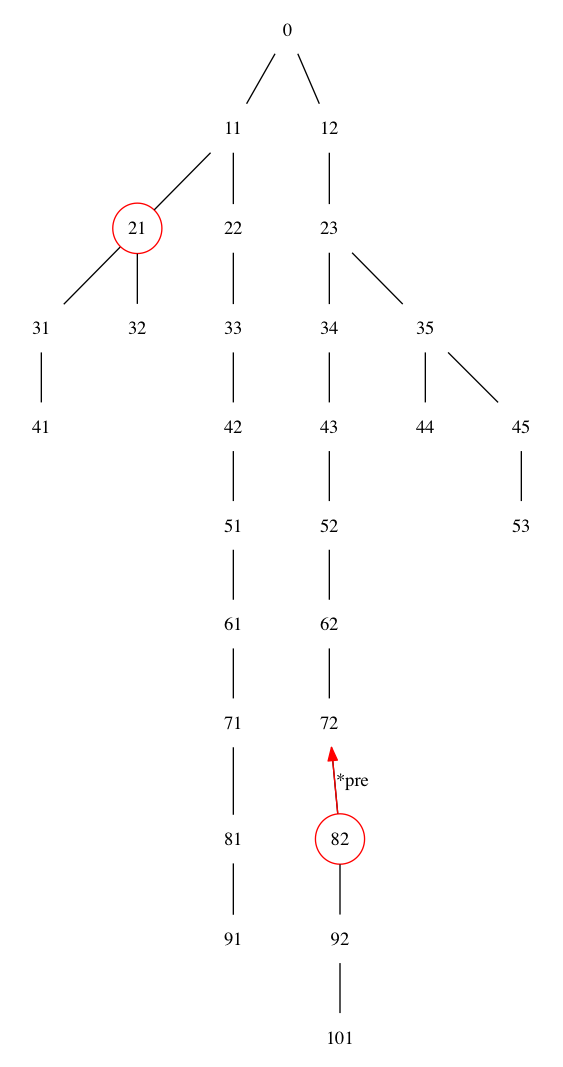
\includegraphics[scale=0.2]{tree.png}
	}
	\subfloat[$k^{1}$ tree]{
		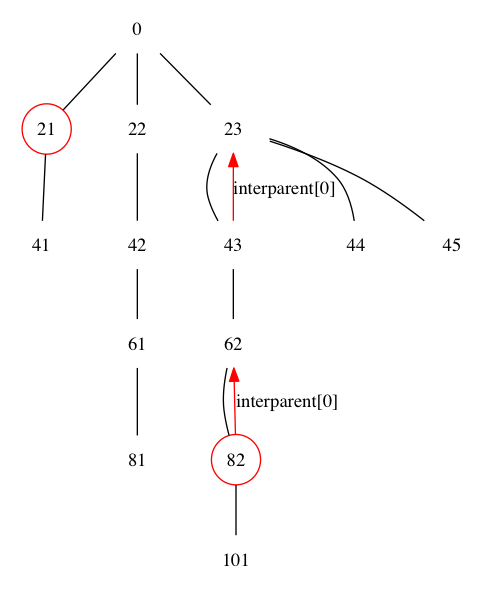
\includegraphics[scale=0.3]{tree1.png}
	}
	\subfloat[$k^{2}$ tree]{
		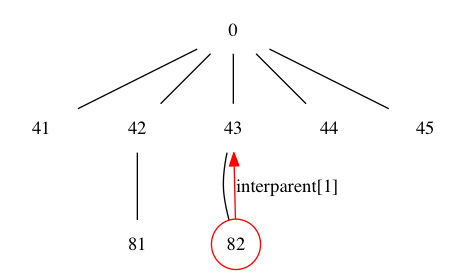
\includegraphics[scale=0.3]{tree2.png}
	}
	
	\caption{Trees with k=2 \label{fig:example}}
\end{figure}

Tree are divided into layers whose events have the same depth and are in immediate conflict.
$e$ and $e'$ are two events in that tree at depths $e.depth$ and $e'.depth$ respectively.
\begin{itemize}
	\item
	If \verb!e.depth = e'.depth!, then $e \icfl e'$
	\item
	If \verb!e.depth! $\neq$ \verb!e'.depth!, without loss of any generality, assume  \verb!depth(e) > depth(e')! . Find an event \verb!e": e" < e! and \verb!e".depth = e'.depth! . If $e" \equiv e'$, then $e'$ and $e$ are in causality, else they are in conflict.
\end{itemize}

\noindent
To quickly find $e"$ through a tree, we apply the idea of skip list (see Fig.\ref{fig:example} for illustration).
Accordingly, in each node, a list of skip predecessors $
skip\_preds = (i_1, i_2,..,i_m)$ are stored, where $i_j$ $(j \in [1,m] )$ is the causal predecessor in $k^{j}$ distance of depth, $k$ $(k > 1)$ is a constant distance in depth which is choosen manually (by experience) to skip through a tree.\\

\noindent
\textbf{Data structure:}
To apply the algorithm of skip list to layered trees, we use a two template class \verb!Node<T,S,SS>! \verb!MultiNode<T,S,SS>! (T is Event) which has the following attributes:
\begin{enumerate}
\item 
	Template struct \verb!Node<T,S,SS>:!
	\begin{itemize}
		\item \textit{depth}: the distance from the root
		\item \textit{*pre}: points to immediate causal predecessor of type T (\verb!pre-proc! or \verb!pre_mem! in Event class)
		\item \textit{skip\_preds}: list of pointers to its $k$-skip predecessors of type T.	
		(T can be an event in the same process or touching the same variable)
	\end{itemize}
\item
	Class template \verb!MultiNode<T,S,SS>!
	\begin{itemize}
	\item
		A list of two \verb!Node!s, repectively corresponding to process and variable nodes.
	\item
		A template function $pred()$ to locate the immediate causal predecessor corresponding to type of \verb!Node!
	\item
		S: 
	\item
		SS: skip
	\end{itemize}
\end{enumerate}

\noindent
Class Event inherits \verb!MultiNode<T,S,SS>! and has two template functions indicating the type of Node.
\begin{itemize}
\item
	\verb!Node<Event> &proc!: return node in equivalent \textit{process} tree
\item	
	\verb!Node<Event> &var!: return node in equivalent \textit{variable} tree 	
\end{itemize}

\noindent
\textbf{Initialize a list of skip predecessors} \verb!skip_preds:!
\begin{enumerate}
\item
	Define the size $s$ of vector \verb!skip_preds! of a node. It depends on the depth of the node.
	
	$s = max(i \in [1,\infty]: e.depth \mod k^{i} = 0 )$ 
\item
	Compute the entire list of skip predecessors for e. For every node, $e.skip\_preds[i]$ is a predecessor at a depth distance of $k^{i}$ from e, so that:
	\begin{itemize}
	\item
		The first element of the list \verb!skip_preds[0]! points to the predecessor at a depth distance of $k^1 = k$ which can be reached by backtracking with $pre$ (actually \verb!e.pre_proc! or \verb!e.pre_mem!)
	\item
		For $\forall i \in [1,s]: skip\_preds[i] = max(\{e": e" < e$ and $e".depth \mod k^i = 0\})$ which can be computed by recursively exploring $k$ times with $skip\_preds[i-1]$: \\
		\verb!e.skip_preds[i] = e.skip_preds[i-1]....skip_preds[i-1]! (k times) 
	\end{itemize}
\end{enumerate}

\begin{algorithm}
	\noindent
	Assume $e.depth > e'.depth$, and , to reach e', do as follows:
	\begin{enumerate}
		\item
		\verb!Set next = e!
		\item
		\verb!while! $next.depth \neq e'.depth$ \verb!do!
		\begin{itemize}
			\item
			\verb!Set d  = next.depth - e'.depth!
			\item
			\verb!Set i  = 0!
			\item
			\verb!while! ($ next.depth \mod k^{i} = 0$)   \space \verb!do!
			$i = i + 1$
			\item
			\verb!Set! $next = next.skip\_preds[i]$ 
		\end{itemize} 
		\item 
		If $next \equiv e'$ then 
		$e'< e$ 
		
		else $e'\cfl e$	 
	\end{enumerate}
	\caption{Decide the conflict between e and e' in the same tree}
	\label{a:layer_tree}	
\end{algorithm}

\begin{algorithm}
	Given two reads $e$ and $e'$.
	\begin{enumerate}
		\item
		Set \verb!w1 = e.find_WR_pred() !
		\verb!w2 = e'.find_WR_pred()!
		\item
		If $w_1 == w_2$
		return false;
		\item
		If $w_1 \cfl w_2$
		return true;
		\item
		If $w_2$ is a successor of $w_1$
		\begin{itemize}
			\item
			Set $w'$ is WR predecessor of $w_2$ at the $w_1.depth + 1$
			\item
			Set $r_1$ = \verb!w'.pre_preaders[e->trans->proc.id]!
			\item
			If ($e$ < $r_1$) then $\lnot (e \cfl e')$
			
			else 	$e \cfl e'$;
		\end{itemize}
		else
		\begin{itemize}
			\item
			Set $w'$ is WR predecessor of $w_1$ at the $w_2.depth + 1$
			\item
			Set $r_1$ = \verb!w'.pre_preaders[e'->trans->proc.id]!
			\item
			If ($e'$ < $r_1$) then $\lnot (e \cfl e')$
			
			else 	$e \cfl e'$;
		\end{itemize}
		
	\end{enumerate}
	\caption{Decide the conflict between two RDs}
	\label{a:rds}	
\end{algorithm}

\begin{algorithm}
	Given two events $e$ is a WR and $e'$ is a RD
	\begin{enumerate}
	\item
		Set 	\verb!w2 = e'.find_WR_pred()!
	\item
		If $e \equiv w_2$
		return false;
	\item
		If $e \cfl w_2$
		return true;
	\item
		If $w_2$ is a successor of $e$, then $e < e'$
	\item
		Else
		\begin{itemize}
			\item
			Set $w'$ is WR predecessor at the $w_2.depth + 1$
			\item
			Set $r_1 = w'.pre\_preaders[e'->trans->proc.id]$
			\item
			If ($e'$ < $r_1$) then $\lnot (e \cfl e')$
			
			else 	$e \cfl e'$;
		\end{itemize}
		
	\end{enumerate}
	\caption{Decide the conflict between a WR and a RD}
	\label{a:wrd}	
\end{algorithm}

\begin{algorithm}
	Given two events touching different variables or 2 LOCs $e$ and $e'$.
	Do the following:
	\begin{enumerate}
		\item
		For each pair $(e_i, e_i')$ of maximal events of each process:
		$e_i \in$ \verb!e.proc_maxevt! and $e_i' \in$ \verb!e'.proc_maxevt! do: \\
		\begin{itemize}
			\item
			If $e_i$.\verb!check_conflict_same_tree(!$e_i'$ \verb!)! is $true$, then  return true;
			\item
			Else jump to 2
		\end{itemize}
		
		\item
		For each pair $(e_i, e_i')$ of maximal events of each process:
		$e_i \in $ \verb!e.var_maxevt! and $e_i' \in$ \verb!e'.var_maxevt! do:\\
		\begin{itemize}
			\item
			If $e_i$.\verb!check_conflict_same_tree(!$e_i'$ \verb!)! is $true$, then  return true;
			\item
			Else, return false;
		\end{itemize}
		
	\end{enumerate}
	\caption{Decide the conflict between 2 LOCs}
	\label{a:arb}	
\end{algorithm}


\section{Unfolding construction}
The algorithm to build the unfolding is to firstly explore a configuration from the bottom (initial state of system) by adding one by one enabled events until reaching maximal events (there is no event enable at the state). At that place, we try to find an alternative to some event in the configuration. There may be a number of such alternatives but we take the very first found one to explore, the rest can be discovered in the coming times.
The exploration can be described as the following: 
\begin{enumerate}
\item 
	From the bottom ($C = \{\bot\}$), extend C by adding one of enabled events at the state of C (initial state at the beginning) until we reach a maximal one.
\item
	Compute conflict extension for maximal configuration C (details in \cref{s:cex}).
\item
	Find an alternative to D after C by judging all combinations of events which are in direct conflict with
	events in D individually. A combination is considered satisfied if it is conflict-free and causal-closed which means it
	forms a configuration.
\item
	If a configuration J is found, extend C by J and repeat the exploration in Step 1 for new configuration.
\item
	If no alternative is figured out, move one of maximal events in C to D, then repeat step 2.
\item
	The exploration termines when no event is enabled
\end{enumerate}

\subsection{Conflict extensions \label{subsec:cex}}

Function \verb!compute_cex! computes conflict extension to a configuration C by generating all possible conflicting events for each one in C. Based on the type of transition an event is labelled with, either RD, WR or SYN, we have separate algorithms. 

\subsubsection{WR conflicting events}
\label{subsection:cex_wr}
\noindent
To compute all events that conflict with a WR event $e$ labelled with transition $t$, do as the following:

\begin{enumerate}
\item Set \verb!ep = e->pre_proc!
\item
	Use function \verb!compute_maxevt()! \cref{a:max} to locate \verb!max_varevt!, the set of maximal events touching variable $t \rightarrow var$ in history of $[ep]$. 
\item Set \verb!ew = e!
\item If $\verb!ew! < \verb!ep!$, then goto End.
\item Let $c \eqdef \tup{s_1, \ldots, s_n}$ be the comb associated to \verb!ew!
	\begin{itemize}
	\item
		Set up the comb whose $spikes[i]$ is a set of RD and WR events that are found by recursively exploring the
		pointer \verb!pre_readers[i]! until the first event of type \verb!WR! or bottom is found.
	\item
		Remove from spikes those that precede any event in \verb!max_varevt! (computed previously), to assure the condition: None of events in $\set{e_1, \ldots, e_n} $ is a causal predecessor of some event in $[ep]$
	\item
		Remember to check empty spikes whenever doing removal on the comb.
\end{itemize}
\item
  Enumerate all combinations $\tup{e_1, \ldots, e_n}$ of $c$ by recursive algorithm.
  For any of them, do:
  \begin{enumerate}
  \item
    If $\tup{e_1, \ldots, e_n} = \verb!e->pre_readers!$, then discard and take
    next one.
  \item
    Create (or retrieve) an event \verb!ex! such that
    \begin{itemize}
    \item \verb!ex->trans = t!,
    \item \verb!ex->pre_proc = ep!,
    \item \verb!ex->pre_readers = {e_1, ..., e_n}!,
    \item \verb!ex->pre_mem = pm! (pm is the first WR found by recursively tracking with pointer \verb!pre_mem!)
    \end{itemize}
  \item
  	Check \verb!ex!'s existence in unfolding with function $find\_or\_add()$. If there does not exist an
  	event in the unfolding having the same \verb!Ident!, add \verb!ex! to the unfolding.
  \item
  	New event created in the unfolding will be added to \verb!cex!. If \verb!ex! is already in the
  	unfolding, it is definitely already in the \verb!cex!
  \item
  	Update \verb!dicfl! (set of directly conflicting events) for both \verb!ex! and other events which are in
  	immediate conflict with it. Refer \cref{a:dicfl} to see the algorithm.
  \item
    Set \verb!ew! = spikes[0].back() 
  \end{enumerate}
\item Goto 3.
\item End.
\end{enumerate}

\begin{algorithm}
	The purpose of the function is to find out all maximal events in calling event's history which read or
	write variable $var$. The resulting events are stored in a vector (std::vector) refered by $max\_varevt
	$.  
	\begin{enumerate}
	\item
		For each process $i$, starting from \verb!ee.proc_maxevt[i]!, backtrack by pointer \verb!pre_proc!
		until we reach bottom or the first event $pm$ that reads or writes variable $t \rightarrow var$.	
	\item
		Push it to \verb!max_varevt!.
	\end{enumerate}
\caption{Function compute maxevt \label{a:max}}
\end{algorithm}

\begin{algorithm}
	Given new conficting event \verb!ex! previously computed in $WR\_cex$ algorithm, the problem is to figure out which of \verb!pre_proc!, \verb!pre_mem! and \verb!pre_readers! are in direct conflict with \verb!ex!. 
\begin{itemize}
\item
	\verb!pre_proc! has no conflict with \verb!ex!
\item
	\verb!pre_mem! is not considered  in issue of conflict.
\item
	For each \verb!ex.pre_readers[i]!, do as the following:
	\begin{itemize}
	\item
		If \verb!ex.pre_readers[i] == e.pre_readers[i]!, then there's no event in conflict with \verb!ex!
		in \verb!i! branch. 
	\item
		If \verb!ex.pre_readers[i] < e.pre_readers[i]!, find \verb!ex!'s immediate successor \verb!es! by recursively tracking from \verb!e.pre_readers[i]!. Add \verb!ex! to \verb!es.dicfl! and reverse.
	\end{itemize}	 
\end{itemize}	
\label{a: dicfl}
\caption{Add to set of immediate conflict events}
\end{algorithm}

\subsubsection{RD conflicting events}
\label{subsection:cex_rd}
For each event $e \in C$ such that \verb!e->trans == t!, repeat the following:
\begin{enumerate}
\item Set \verb!ep = e->pre_proc!
\item Set \verb!em = e->pre_mem!
\item If $\verb!em! < \verb!ep!$, then goto End.
\item If \verb!em! is \verb!RD!, then set \verb!em = em->pre_mem!
\item If not, it must necessarily be \verb!WR!; then set \verb!em = em->pre_readers[t->proc]!
\item (Warning: check for the bottom event in previous calculation)
\item
  Create (or retrieve) an event \verb!ex! such that
  \begin{itemize}
  \item \verb!ex->trans = t!,
  \item \verb!ex->pre_proc = ep!,
  \item \verb!ex->pre_mem = em!,
  \end{itemize}
  
\item Check if \verb!ex! is enabled at the new local configuration
\item Event \verb!ex! is in $\cex C$
\item Goto 4.
\item End.
\end{enumerate}

\subsubsection{SYN conflicting events}
\label{subsection:cex_syn}
\noindent
It is noticable for SYN events that an UNLOCK event can only be enabled from a LOCK and reverse.
For each event $e \in C$ such that \verb!e->trans == t!, repeat the following:
\begin{enumerate}
\item Set \verb!ep = e->pre_proc!
\item Set \verb!em = e->pre_mem!
\item If  \verb!em < ep!, then goto End.
\item Set \verb!em = em->pre_mem->pre_mem! (skip the \verb!pre_mem! which does not have the same type of SYN)
\item (Warning: check for the bottom event in previous calculation)
\item
  If \verb!t! is enabled at the state of $[ep] \cup [em]$, then create (or retrieve) an event \verb!ex! such that
  \begin{itemize}
  \item \verb!ex->trans = t!,
  \item \verb!ex->pre_proc = ep!,
  \item \verb!ex->pre_mem = em!,
  \end{itemize}
\item Event \verb!ex! is in $\cex C$
\item Goto 3.
\item End.
\end{enumerate}

\subsection{Alternative}
\noindent
Given a configuration $C \subseteq U$ and a set of events $D \subset U$, an alternative to D after C is an configuration $J \subset U $ such that:

\begin{flalign}
C \cup J \text{ is a configuration} \label{eq1}\\
\text{For all event } e \in D \text{, there is some } e'\in C \cup J \text{ such that } e' \in  \icfl \{e\}  	\label{eq2}
\end{flalign}



\noindent
We know that $\forall e \in D: $ $e \in cex(C)$ or $e \in en(C)$. Therefore, $\forall e \in D: e \in cex(C)$ (computed in \cref{subsec:cex}), there exists an event $e' \in C: e' \icfl e$ which implies that $e$ is definitely satisfied and then it should not be taken into account. In the other case, $e \notin cex(C)$, do as follows to find out a J if it exists:

\begin{itemize}
\item 
	$A = \{e_i \in D: e_i \in en(C)\}$ (A is a D prunned any event in $cex(C)$). 
	Set up a \emph{comb} (over A),
	an $n$-tuple $c \eqdef \tup{s_1, \ldots, s_n}$ of sequences $s_i \in A^*$
	($i \in  \set{0,\ldots ,n}$ with $n = \left\vert{A} \right\vert$).
	Each sequence $s_i$ is called a \emph{spike} 
	which contains all events that are in immediate conflict with $e_{i} \in A$ (see \cref{a:dicfl} for direct conflict checking algorithm).
	If there is an empty spike, $e_i$ has no conflicting event, then there exists no J.
\item
	Given a comb $c$ witout any empty spike, a \emph{combination} over $c$ is any $n$-tuple $a = \tup{e_1, \ldots, e_n} \in A^n$ such that $e_i \in A$ is one element of the sequence $s_i \in A^*$, for $i \in \set{1, \ldots, n}$. \\
	$a$ is an alternative we are looking for if it holds both \eqref{eq1} and \eqref{eq2} in the definition: 	
\begin{itemize}
	\item
		If $\exists e_i \in a$: $e_i \cup C$ is not a configuration, it means \eqref{eq1} condition is not satisfied, then discard the combination.
	\item
		If \eqref{eq1} holds, check whether $a$ is conflict-free which means there is not any pair of event $(e_i, e_j)$ in conflict (see ...for conflict checking algorithm):
		\begin{itemize}
			\item
				If there exist a pair $(e_i, e_j)$ such that $e_i \cfl e_j$, discard the combination.
			\item
				If not, (2) condition is definitely satisfied. By then, J is formed as the union of local configurations of all events in $a$:
				\begin{equation}
				\nonumber
					J = \cup [e_i] \text{ with } \forall  e_i \in a
				\end{equation}
				 
		\end{itemize}
\end{itemize}
\end{itemize}


\begin{algorithm}
To find out an alternative to D after C, do as follows:
\begin{enumerate}
	\item
	Remove from D all events in cex(C). 
	\item
	Let $comb \eqdef \tup{s_1, \ldots, s_n}$ be the comb over D where 
	$s_i$ is a set of events in direct conflict with $e_i$: $s_i$ = $e_i \rightarrow$ \verb!dicfl!
	\item
	Remove from the $comb$ all events that are in conflict with any maximal event of C. If the removal leaves some empty spike, 
	there obviously exists no alternative, so go to End
	\item
	Enumerate all combinations $\tup{e_1, \ldots, e_n}$ of $c$.
	\item
	For any of them, do:
	\begin{itemize}
		\item 
		If $\tup{e_1, \ldots, e_n}$ is conflict-free (use function \verb!check_cfl!), return $J = \cup [e_i]$. (Caution: Remember to remove from J those are already in C.
		\item
		If there exist any conflict among events in J, then discard J and come back to step 2
		to take next combination.
	\end{itemize}
	\item End.
\end{enumerate}
\caption{Computing an alternative J for D after C}
\label{a:alter}
\end{algorithm}


\end{document}
